\documentclass{article}
\usepackage[a4paper, margin=0.5in]{geometry}
\usepackage{enumitem}
\usepackage{graphicx}
\usepackage{placeins}
\usepackage{subcaption}
\usepackage{amsmath}
\usepackage{listings}
\usepackage{color}

\definecolor{commentcolor}{rgb}{0.5,0.5,0.5}
\definecolor{keywordcolor}{rgb}{0,0,1}
\definecolor{stringcolor}{rgb}{0.58,0,0.82}

\lstdefinelanguage{asm}{
    keywords={ldr, str, add, subs, b, mov},
    morecomment=[l]{;},
    sensitive=true,
    morestring=[b]"
}

\lstset{
    basicstyle=\ttfamily\small,
    commentstyle=\color{commentcolor},
    keywordstyle=\color{keywordcolor},
    stringstyle=\color{stringcolor},
    showstringspaces=false,
    breaklines=true,
    frame=single,
    language=asm
}

\begin{document}
\title{Traffic Light Simulation}
\author{Group 32}

\maketitle

This report represents the comprehensive details of our project, which includes the development and implementation of an assembler and our extension in the Raspberry Pi. This project aims to demonstrate our ability to design, implement, and test a complete system while working collaboratively in a group.

\section{Implementation Details for Part II and Part III}

\subsection{Part II: Assembler Structure and Implementation}
The main new structure we defined for the assembler is the symbol entry and symbol table, which is shown below:



\begin{minipage}{0.45\textwidth}
\begin{lstlisting}[language=C, caption=Symbol Entry]
typedef struct symbol_entry {
    dynamic_string *label;
    uint64_t address;
} symbol_entry;
\end{lstlisting}
\end{minipage}
\hfill
\begin{minipage}{0.45\textwidth}
\begin{lstlisting}[language=C, caption=Symbol Table]
typedef struct symbol_table {
    symbol_entry **symbols;
    size_t size;
    size_t capacity;
} symbol_table;

\end{lstlisting}
\end{minipage}

The symbol entry consists of a label and an address. The label is a \verb|dynamic_string|, which is a custom data structure we made to allow us to store strings of any size. This is because labels could be of arbitrary length, so we had no guarantee that a string label would fit in a fixed-capacity array. This required a bit more work, but means that our implementation is correct for any given label. The symbol table contains an array of pointers to symbol entries, as well as a size and capacity to keep track of how many symbols we are using, allowing us to \verb|realloc| when size equals capacity. 

Another key structure is the instruction, which was initialised during the parser stage. It identified the line number and label, as well as the opcode and operands. This is all the necessary information for encoding the instruction, and thus we only passed one argument to the instruction handlers.

We also quickly identified aspects of our code that multiple people relied on. For example, it was beneficial to establish an array of strings containing all the valid opcodes, since various parts of the code needed to identify the type of instruction. Thus, we extracted this into a separate file, which eliminated redundancy.


\subsection{Part III: Implementing the Red LED Blink Task on the Raspberry Pi}

Using the assembler from the previous part, we wrote assembly code to achieve the task of blinking the LED on the Raspberry Pi.
\subsubsection{Initialisation and Setting the GPIO Pin}

The code begins by initialising several registers with the addresses of the GPIO memory locations and specific values needed for controlling the GPIO pin.

\begin{minipage}{0.45\textwidth}
\begin{lstlisting}[language=asm, caption=Blink LED Initialisation]
ldr w21 gpio21
ldr w22 setup_gpio
str w21 [x22]
ldr w18 clear_gpio
ldr w19 set_gpio
ldr w20 bit21
\end{lstlisting}
\end{minipage}
\hfill
\begin{minipage}{0.45\textwidth}
\begin{lstlisting}[language=asm, caption=GPIO Pin Set]
set:
str wzr [x18]
str w20 [x19]
\end{lstlisting}
\end{minipage}

\begin{enumerate}[itemsep=0.5mm]
    \item \verb|w21| is loaded with the value from \verb|gpio21|, which contains the pin number for GPIO21.
    \item \verb|w22| is loaded with the address of \verb|setup_gpio|, which contains the memory address for the GPIO Function Select Register for setting the pin mode. The value in \verb|w21| is stored at the address pointed to by \verb|x22|, effectively setting the GPIO21 pin to output mode.
    \item \verb|w18|, \verb|w19|, and \verb|w20| are loaded with addresses for clearing, setting, and the bit mask for GPIO21, respectively.
    \item At the label \verb|set|, the code first stores the zero register (\verb|wzr|) at the address in \verb|x18| to ensure any previous state is cleared.
    \item It then stores the value in \verb|w20| at the address in \verb|x19| to set the GPIO pin high.
\end{enumerate}

\subsubsection{Creating a Visible Blink and Swapping Registers}

\begin{minipage}{0.45\textwidth}
\begin{lstlisting}[language=asm, caption=Delay Loops]
delay:
    add x28, x28, #10000
delay_outer_loop:
    add x29, x29, #1000000
delay_inner_loop:
    subs x29, x29, #1
    b.ne delay_inner_loop
subs x28, x28, #1
b.ne delay_outer_loop
\end{lstlisting}
\end{minipage}
\hfill
\begin{minipage}{0.45\textwidth}
\begin{lstlisting}[language=asm, caption=x18 and x19 Swapping]
mov x17 x18
mov x18 x19
mov x19 x17
b set
\end{lstlisting}
\end{minipage}

\begin{enumerate}[itemsep=0.5mm]
    \item The delay loops are implemented using two nested loops to achieve the necessary 10 billion iterations before changing the LED state, a number too large for a 32-bit signed integer.
    \item The nested loop structure ensures a substantial delay, as the cumulative number of iterations is high enough to create a visible blink.
    \item After the delay, the code swaps the contents of registers \verb|x18| and \verb|x19| to invert the action for the next loop iteration.
    \item The code then branches back to the \verb|set| label to repeat the process, creating an infinite loop of toggling the GPIO pin state.
\end{enumerate}

\subsubsection{Data Section}
The data section at the end of the code defines the memory addresses and values used.\par\medskip 
\noindent
\begin{minipage}{0.45\textwidth}
\begin{lstlisting}[language=asm, caption=GPIO Setup]
setup_gpio:                     
    .int 0x3f200008 ; Address for GPIO Function Select register            
clear_gpio:                    
    .int 0x3f200028 ; Address for GPIO Clear register                             
set_gpio:                          
    .int 0x3f20001c ; Address for GPIO Set register                
\end{lstlisting}
\end{minipage}
\hfill
\begin{minipage}{0.45\textwidth}
\begin{lstlisting}[language=asm, caption=GPIO Constants]
gpio21:
    .int 0x8        ; GPIO21 pin number
bit21:
    .int 0x200000   ; Bit mask for GPIO21
zero:
    .int 0x0        ; Zero value for initialisation. Used for clearing registers before loop
\end{lstlisting}
\end{minipage}

\section{Extension: Traffic Light Simulation}
\subsection{Thought Process behind the Extension}
\subsubsection{Our Initial Idea and its Challenges}
Initially, we had an interesting idea to create a weather station. However, we encountered several challenges with the concept. Firstly, the sensor we used was not reporting the readings correctly. After some troubleshooting, we discovered that this was due to difficulties interfacing with the hardware, coupled with unclear specifications. This made it difficult to achieve correct readings.

Moreover, the complexity of communicating between the sensors and the Raspberry Pi added another level of difficulty. While we could have added more sensors, the implementation would essentially remain the same, offering little room for substantial progress.

\subsubsection{Switching to the idea of a Traffic Light Simulation}
Given these limitations, we decided to pivot to a different idea: a traffic light simulation. This new concept not only avoided the hardware issues we faced with the weather station but also provided us with the opportunity to be creative and implement meaningful extensions.

\subsection{Overview of the Extension}
We had three main objectives for the extension:

\begin{enumerate}[itemsep=0.5mm]
    \item Simulate a four-way traffic light system with cars approaching randomly from all directions.
    \item Test various algorithms to minimise the overall waiting time for vehicles.
    \item Extend the system to utilise an ultrasonic sensor to provide additional information to the algorithms.
\end{enumerate}

Firstly, we created a representation of the traffic light systems using physical LEDs, simulating a four-way intersection with cars approaching randomly from all directions. To achieve this, we wired and programmed the LED’s to mimic real-world traffic signals. This setup allowed us to create a realistic and functional simulation of a busy intersection.

Secondly, we created various algorithms to minimise the overall waiting times for cars at our intersection. We implemented three traffic management algorithms, and each one was tested for numerous iterations to evaluate its efficiency in reducing wait times.

Lastly, we extended the system to utilise an ultrasonic sensor. The sensor provided additional information to the algorithms in determining when to transition to the next state. The ultrasonic sensor allowed us to detect how close cars were to the stop light, which we used to change the duration of the state. This integration not only enhanced the accuracy of our simulation but also added a layer of complexity that made our project more realistic.

In summary, by focusing on these three objectives, we were able to create a comprehensive and efficient traffic light simulation.


\subsection{Details of the Design}

\subsubsection{Physical LED System}
The setup of the physical LEDs was similar to the blink LED task we performed earlier but with significantly more complex logic. We designed a system that cycled through an order of states, determined by our traffic management algorithms. This involved coordinating the timing and sequence of the red, yellow, and green lights for each direction at the intersection, ensuring that the lights changed in a way that mimicked real-world traffic lights. Simulating cars approaching the intersection involved making several assumptions about their behaviour. For example, we assumed that all cars move at a constant speed whenever there is space in front of them. This assumption allowed us to simplify the logic needed to control the traffic flow and determine the state transitions.

\subsubsection{Various optimising algorithms}
After considering our options for our optimisation problem, we decided to apply four algorithms to our system: \verb|basic|, \verb|basic_plus|, and a \verb|genetic_algorithm| with two variations. The basic function updates the state of the lights based on fixed timings for each road. The basic plus function is similar but accounts for the approach of a vehicle detected by the ultrasonic sensor (using a sigmoid-inspired function) and will only update if cars are waiting for the lights. The functions are shown below:

\begin{lstlisting}[language=C, caption= The strategies and their parameters]
typedef bool (*strategy)(intersection *isec, time_t time_since_change, Chromosome *optimal_data);
bool basic (intersection *isec, time_t time_since_change, Chromosome *optimal_data);
bool basic_plus (intersection *isec, time_t time_since_change, Chromosome *optimal_data);
bool genetic_algorithm (intersection *isec, time_t time_since_change, Chromosome *optimal_data);
\end{lstlisting}

We then implemented two algorithms that allowed the fixed timings to alter, optimising the light change timings. The first algorithm trains based on the average waiting time of cars throughout a whole simulation, whereas the second trains based on the maximum waiting time. This training is accomplished using a machine-learning approach called the genetic algorithm. The genetic algorithm works by having a dataset to optimise, which for us was the duration to hold each state, as well as the “fitness” or performance of that dataset. These are stored in a structure called “chromosome”, and we create an array of these chromosomes to form a “population”. We decided to make the population size 100 to ensure diversity in the durations, and this population initially contains chromosomes with randomised state durations with a maximum duration of 50 and a minimum duration of 1.

We also chose the number of generations, which is the number of times for reconstructing the population, and we decided 10 would be a good number to ensure the best chromosome is chosen. Reconstructing the population will be based on the previous population's best results, with some randomness to ensure the dataset can explore alternative durations. For every new generation, we evaluate the old generation’s performance by running each chromosome through a few simulations of the intersection and averaging the results. We then select parent chromosomes, which will either be a random chromosome from the population or the best chromosome.

Once parent chromosomes have been selected, we either assign these to the next generation or crossover the datasets to generate two child chromosomes depending on the crossover rate, which will then be mutated and form the next generation. After the last generation has been evaluated, the best chromosome from that generation is taken in to be tested further for a more precise performance evaluation. The average and maximum waiting times for the cars are then written into a file for us to evaluate the results.
\begin{lstlisting}[language=C, caption=The structure of the Chromosome]
typedef struct {
    int durations[NUM_STATES];
    double fitness;
} Chromosome;
\end{lstlisting}
\begin{lstlisting}[language=C, caption=The main training loop]
Chromosome train_genetic_algorithm(bool is_avg) {
    Chromosome population[POP_SIZE];
    initialise_population(population);
    for (int generation =  0; generation < MAX_GENERATIONS; generation++) {
        for (int i = 0; i < POP_SIZE; i++) {
            evaluate_fitness(&population[i], is_avg);
        }
        create_new_population(population);
    }
    for (int i = 0; i < POP_SIZE; i++) {
            evaluate_fitness(&population[i], is_avg);
    }
    Chromosome best = get_best_chromosome(population);
    print_chromosome(&best, is_avg);
    return get_best_chromosome(population);
}
\end{lstlisting}
\subsubsection{Ultrasonic Sensor}
We extended the system to utilise an ultrasonic sensor to provide additional information to the algorithms in determining when to transition to the next state. This decision was inspired by our desire to incorporate sensors into our system, enhancing the data available for algorithmic processing. The ultrasonic sensor measures the time between sending out a sound wave and detecting its return, which we converted into a distance using the speed of sound. This distance was then integrated into some of our algorithms to improve their accuracy and responsiveness.
\section{Testing and Effectiveness}
For our system, \verb|basic| and \verb|basic_plus| acted as baselines to measure against. We decided to use them as most traffic lights seem to be using some form of fixed timings.
\subsection{How We Tested Our Extension}
We decided to use the average and maximum time cars are stationary, as well as the total number of cars crossed, to measure the effectiveness of our algorithms. To do this, we made two structures: one for evaluating the performance on a road and the other for the performance on the whole intersection. These values were printed out to a file, and the number of cars was used to plot graphs.
\begin{lstlisting} [language=C, caption=The functions and structures needed to evaluate efffectiveness]
typedef struct {
    time_t total_time_stationary;
    int num_cars_crossed;
    time_t maximum_time_stationary;
} road_evaluation;
typedef struct {
    road_evaluation *road_evals[NUM_ROADS];
    double total_average_time_stationary;
    time_t total_maximum_time_stationary;
} intersection_evaluation;
\end{lstlisting}
\subsection{Results and Effectiveness of Our Extension}

The following is the result of running the simulation for a large number of iterations that we used in the presentation:

\begin{lstlisting}
Strategy: Basic Total Average Time: 6.684007, Total Maximum Time: 39.000000
Strategy: Basic Plus Total Average Time: 6.750644, Total Maximum Time: 39.000000
Strategy: Genetic Algorithm Avg Total Average Time: 0.349173, Total Maximum Time: 7.000000
Strategy: Genetic Algorithm Max Total Average Time: 0.316471, Total Maximum Time: 6.000000
\end{lstlisting}


Note that the results are random by nature, and thus will not be consistent. To account for this, we ran the simulation many times. Therefore, we can confidently say that the genetic algorithm shows around a 20 times lower average time, and 5 times lower maximum time. However, the algorithm produced some unusual state duration timings. The states where some lights are amber were massively prioritised, which occurred because cars are allowed to cross during the amber states. The algorithm could then quickly switch states to green or red. 

The algorithm chose to stay on amber lights for 40 seconds or more! While this achieves a low waiting time for the vehicles, it is not a realistic model. There were two main reasons that this occurred. Firstly, our simulation itself wasn't modelled entirely accurately. This was due to assumptions we made about the cars: modelling them all as the same car, not taking into account acceleration (we modelled the cars to stop instantaneously), and not modelling cars crashing, all of which could have affected the evaluation of each chromosome. Secondly, the function used to evaluate the fitness of a chromosome did not punish the chromosome for having unnatural timings. The combination of these issues resulted in the algorithm consistently finding out that the most effective way of reducing waiting times is keeping lights on amber. To implement this traffic light optimising algorithm in the real world, we would need to fix these issues and ensure there are safeguards.

Turning our attention to the basic plus algorithm, we were surprised that it was marginally worse than the Basic algorithm. The Basic Plus algorithm had more information about the state of the intersection, which we expected to give us better results. However, we believe the fact that the intersection only had one sensor was detrimental. The basic plus algorithm prioritised the road with the sensor above all else when a car approached. It is a good example of a situation where a more complex solution is not the most effective.

We also kept track of the number of cars in the intersection and graphed these results (see Figures (a) and (b) below). According to Figure (a), the genetic algorithms reached a maximum of 18 cars in the intersection, whilst the basic algorithms had a maximum of over 20 cars. Furthermore, there is less variance in the number of cars when using the genetic algorithm. This suggests that the genetic algorithm is more effective at maintaining a consistent traffic flow.

We had four roads that only allowed cars to go straight and with our configuration, only Road 0 had a sensor. As a result, it often had more cars than the other roads, except the road opposite (Road 2) which has the same light state. This is because the sensor identified that the cars have not reached the light yet, so there is no need to switch the light to green. This allowed us to keep the number of cars on the other roads low, without causing delays on the road with the sensor. In Figure (b), we note Road 1 and Road 3 often have zero cars, while the number of cars is more consistent on Road 0 and Road 2.

\FloatBarrier
\begin{figure}[h]
\centering
\begin{subfigure}{0.49\textwidth}
\centering
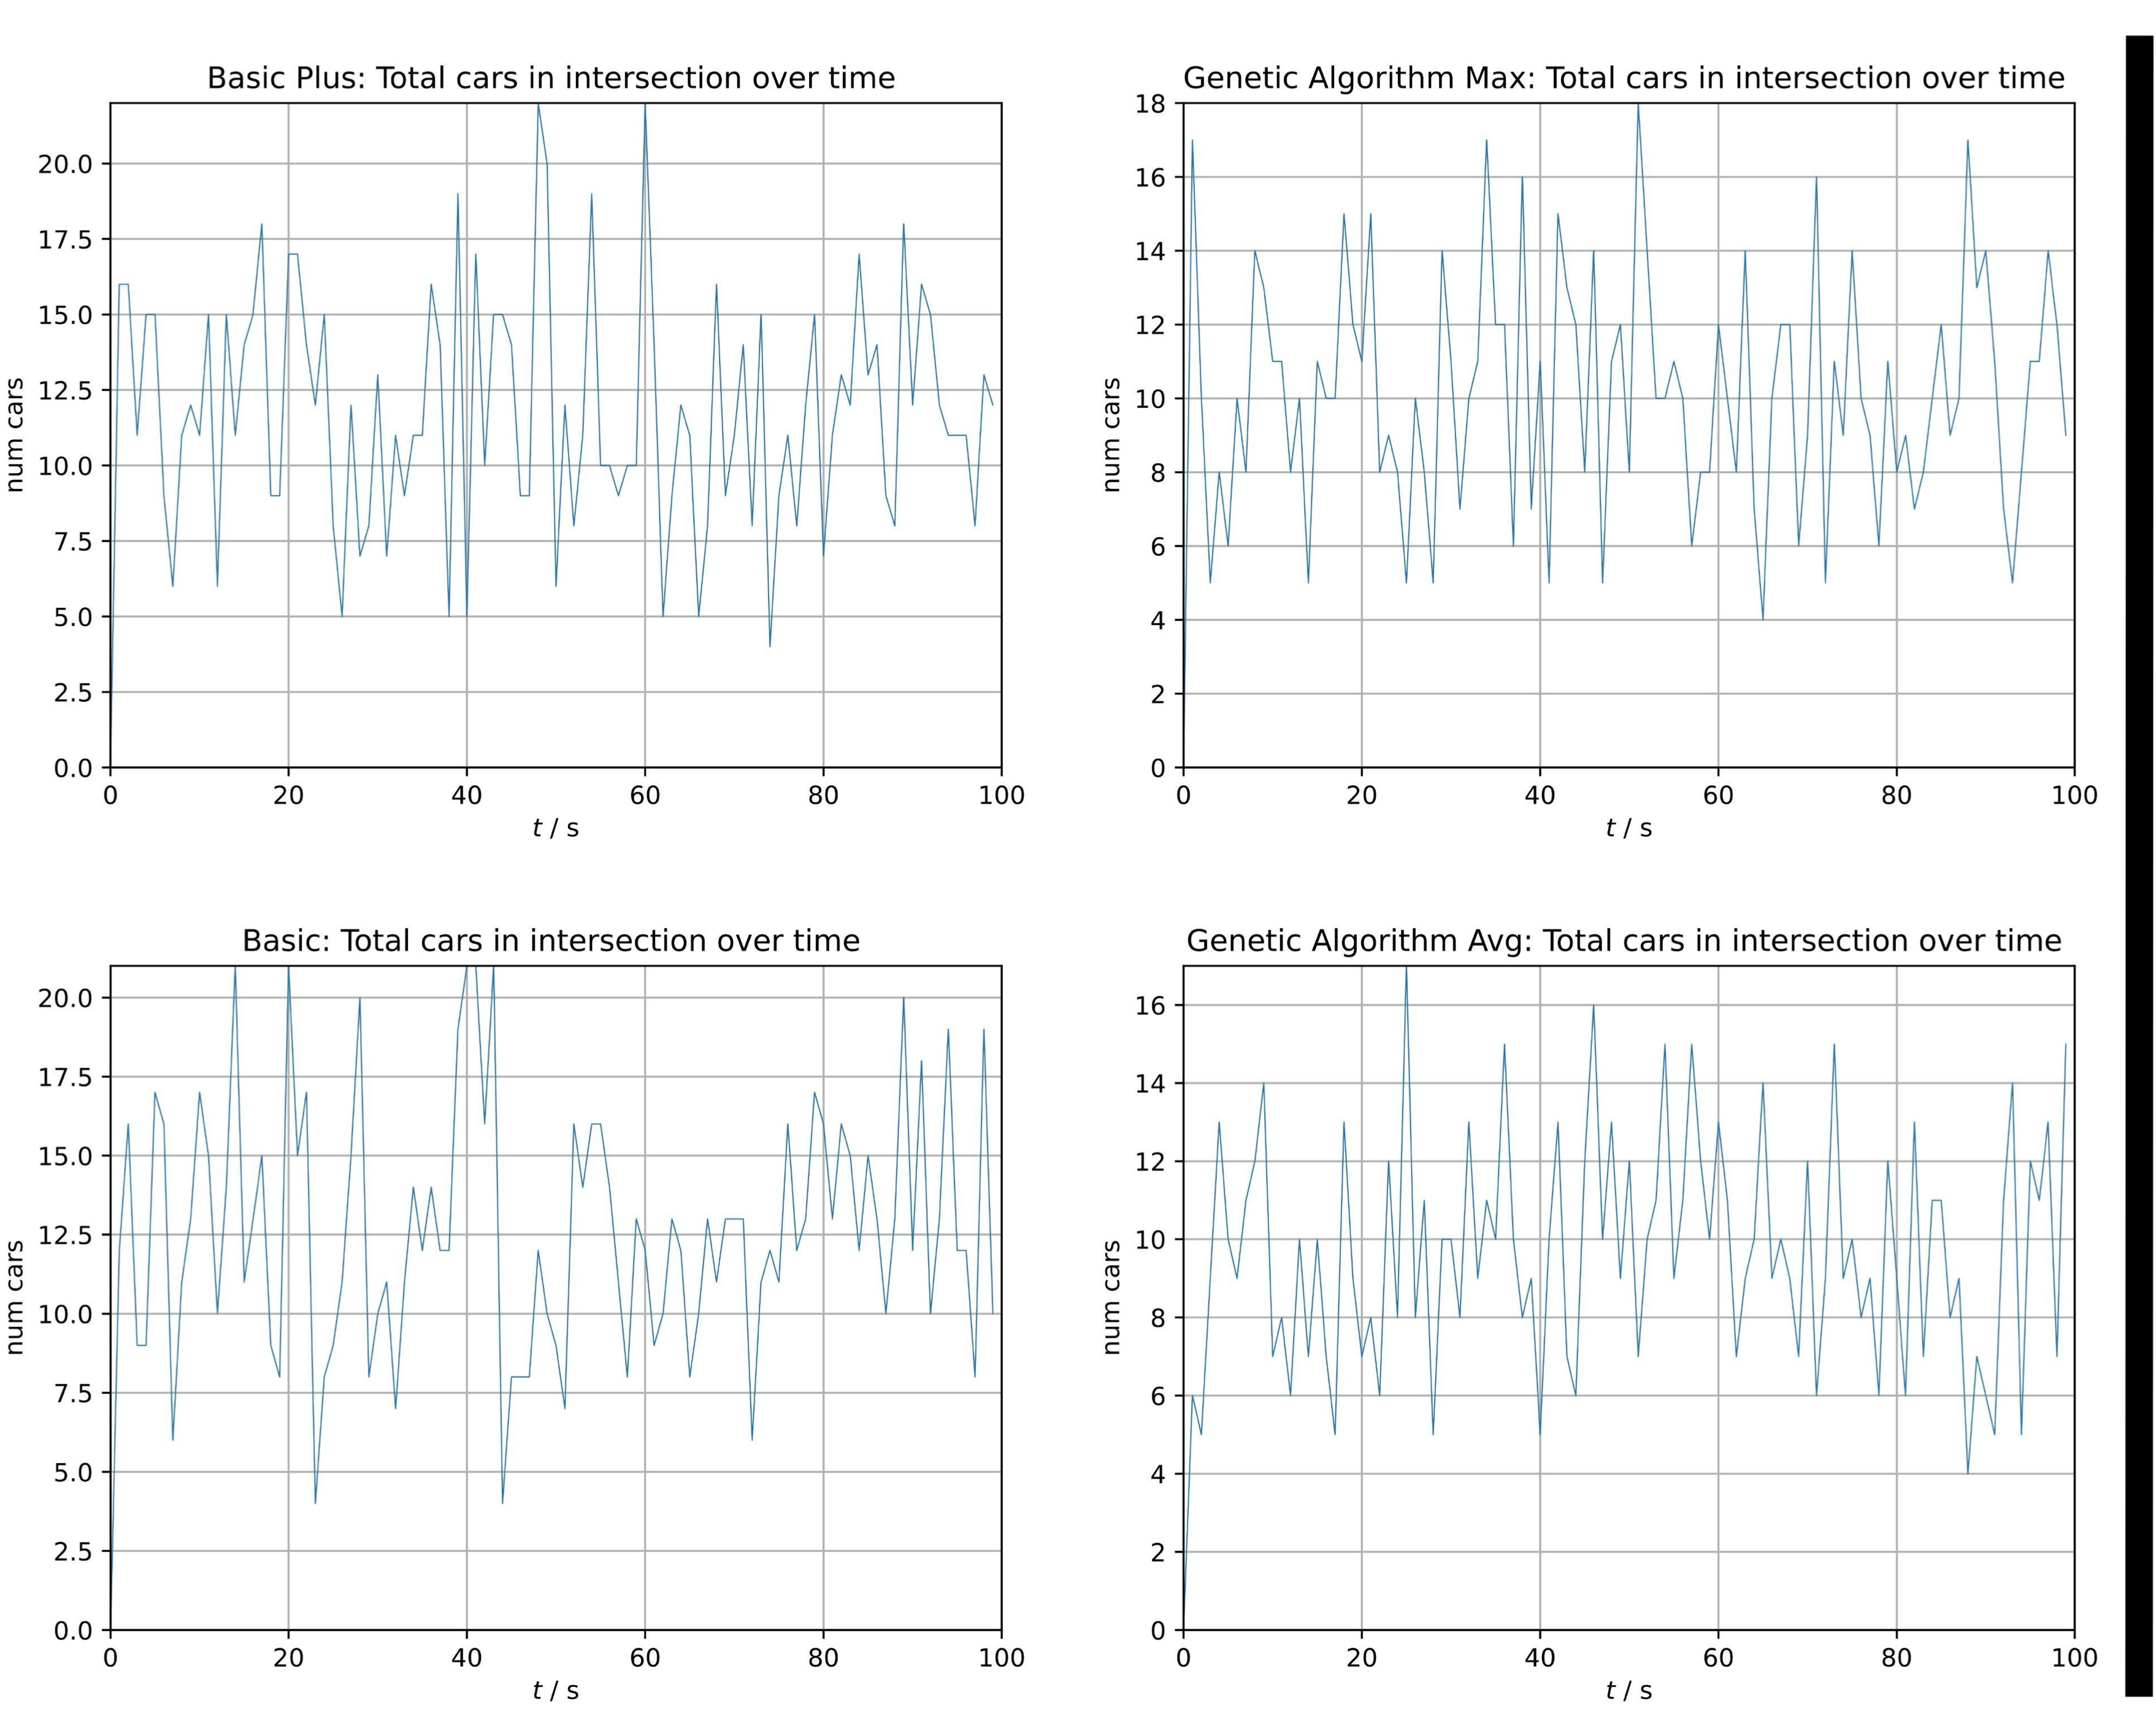
\includegraphics[width = \textwidth]{graph1.png}
\caption{Total cars in intersection for various algorithms}
\label{fig:left}
\end{subfigure}
\begin{subfigure}{0.49\textwidth}
\centering
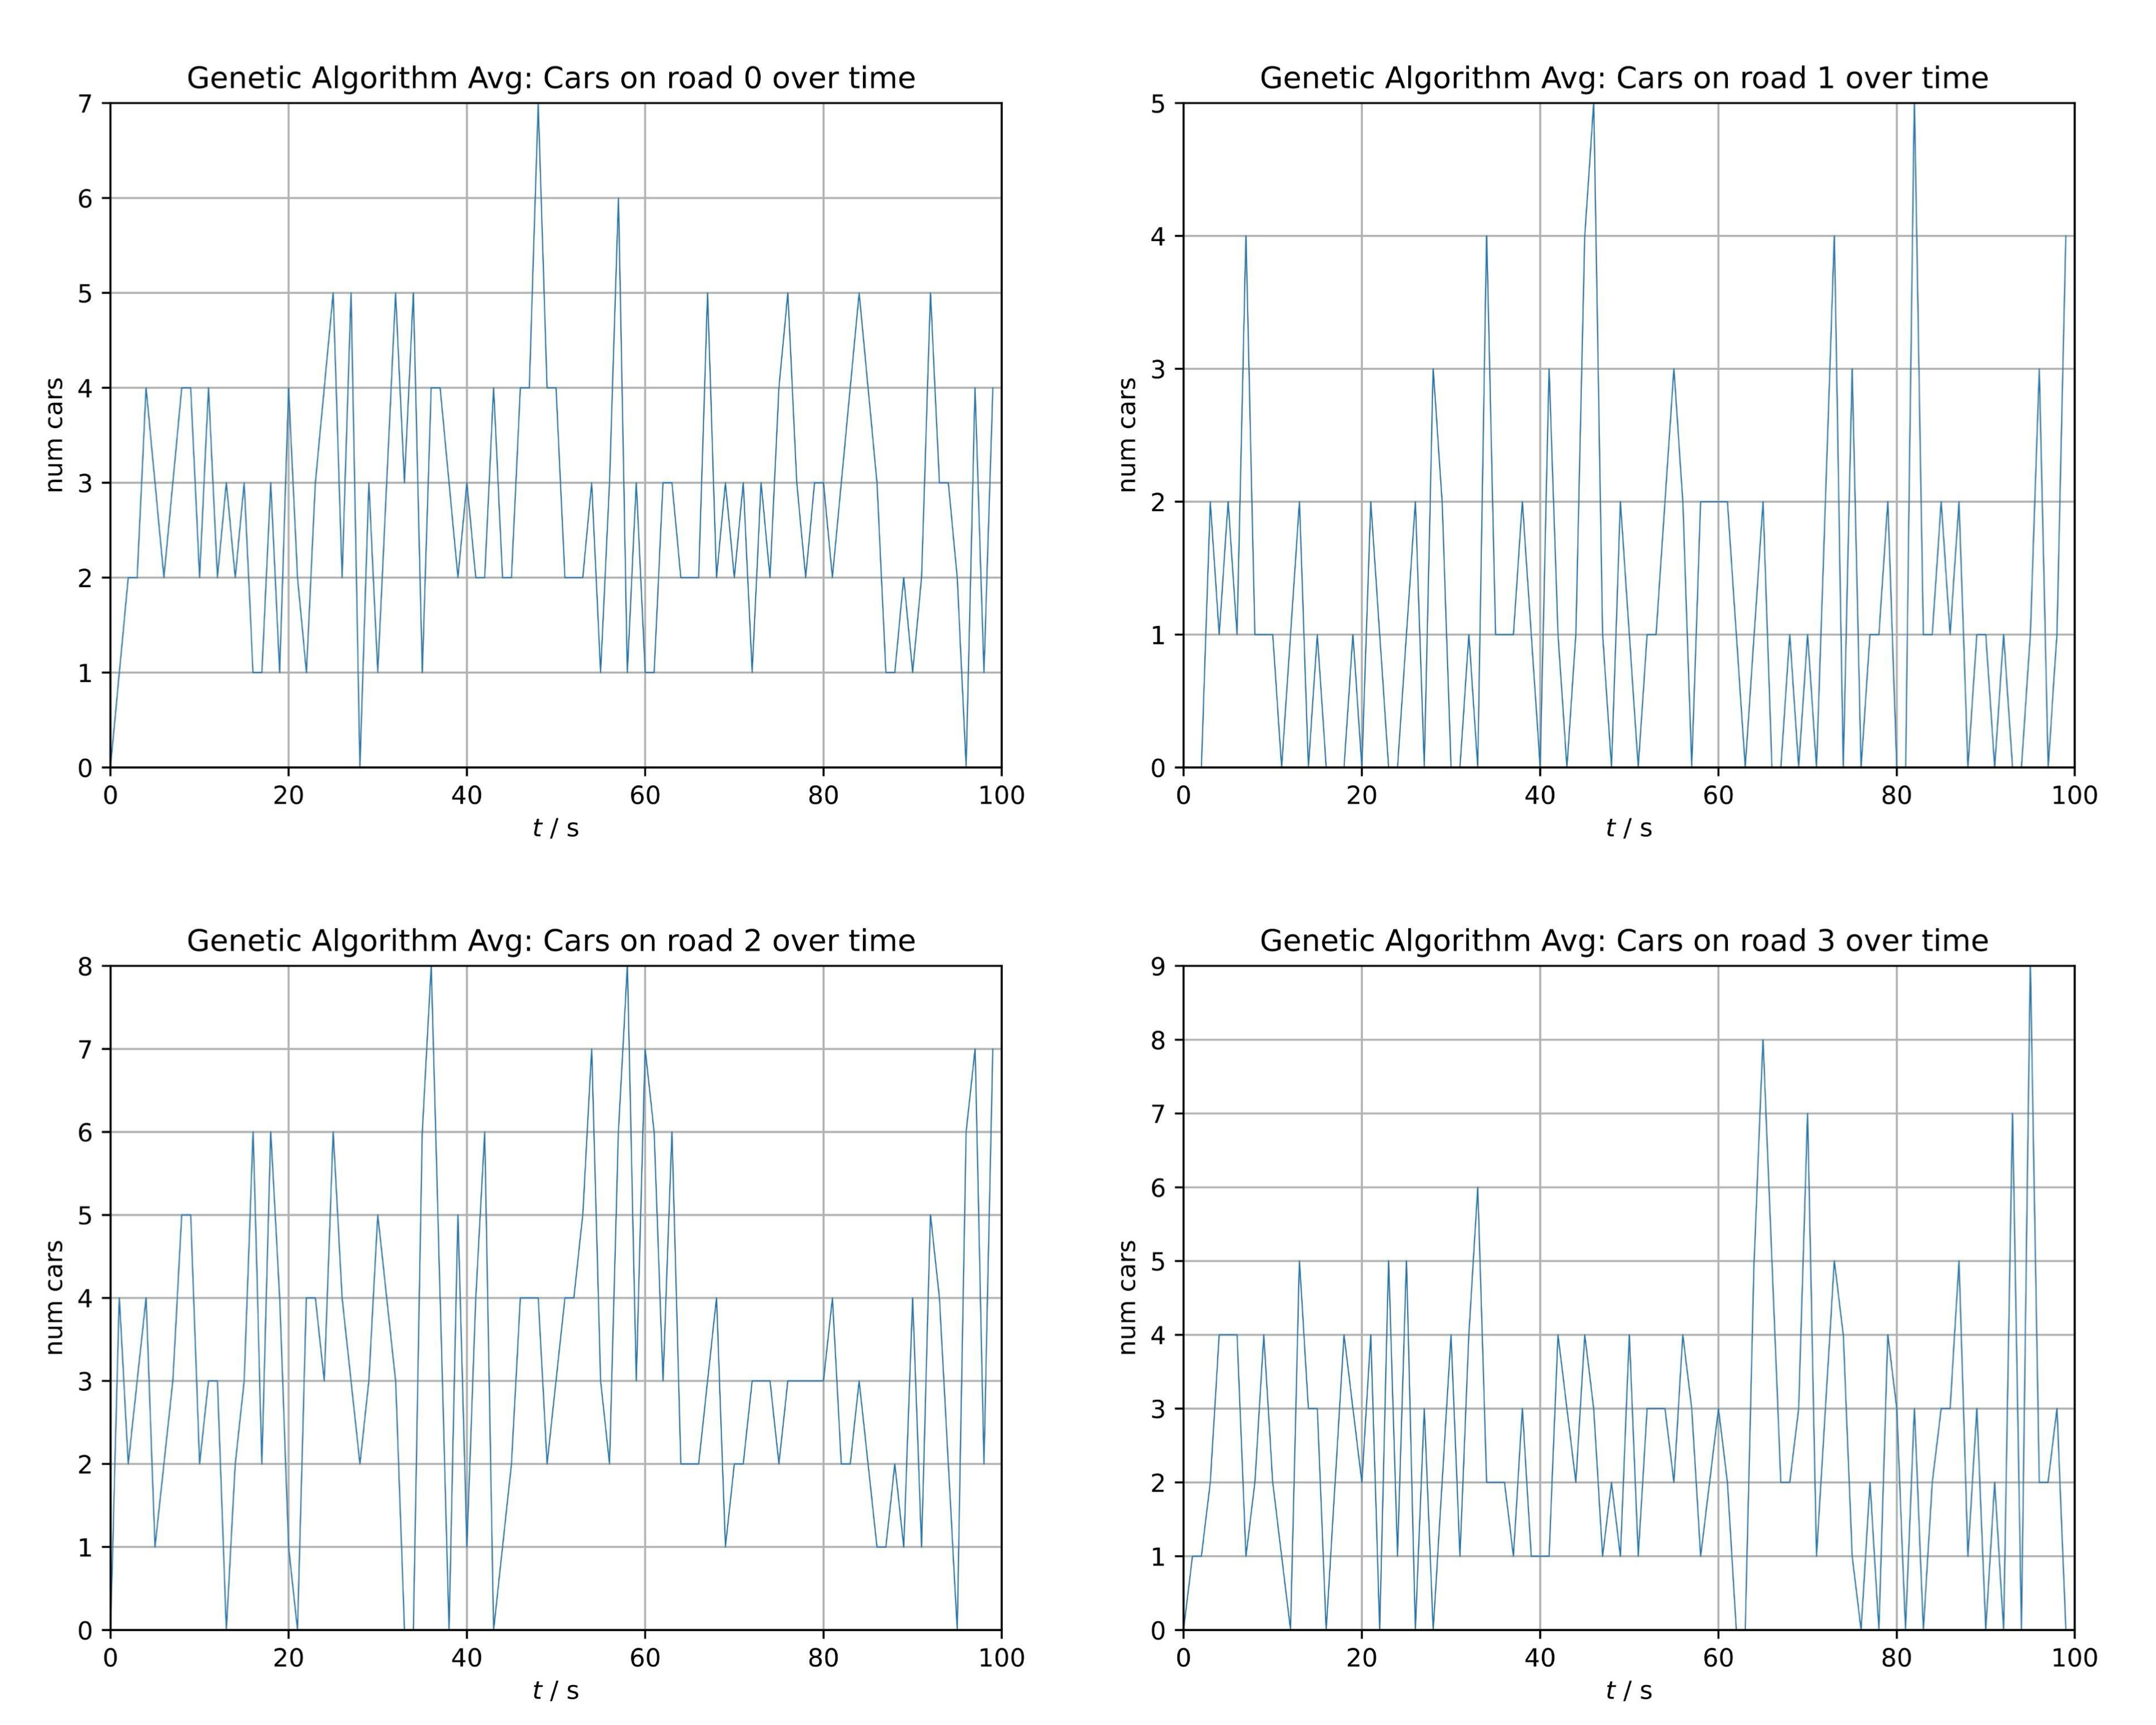
\includegraphics[width = \textwidth]{graph2.png}
\caption{Cars on Roads 0 to 4, Genetic Algorithm}
\label{fig:right}
\end{subfigure}
\label{fig:combined}
\end{figure}

\FloatBarrier


\section{Group Reflection}
\subsection{Effectiveness of Communicating and Splitting Work}
Our initial progress with this programming assignment went smoothly, which gave us confidence moving forward. Throughout the project, we maintained consistent progress and accomplished everything we set out to do for the extension.

We communicated effectively, holding regular meetings and providing updates to ensure everyone was on the same page. We supported each other when we encountered bugs and hurdles, and as the project progressed, everyone contributed equally. Overall, we are happy with the quality of the work produced by the group.

This exercise gave us valuable insights into programming effectively. We learned how to use Git properly and effectively, which was crucial for managing our codebase. Additionally, having different ways of thinking within the group helped us overcome challenges more quickly than if we had worked individually.

\subsection{What We Will Maintain}
We found several practices beneficial that we would like to maintain in future projects:

\begin{enumerate}[itemsep=0.5mm]
    \item Always maintain a global to-do list, breaking it down into individual to-do lists as soon as the tasks are assigned.
    \item Continue with pair programming, as it significantly improved our productivity and code quality.
\end{enumerate}

\subsection{What We Would do Differently}
There are a few things we would do differently in future projects:
\begin{enumerate}[itemsep=0.5mm]
    \item Start pair programming earlier, as this method was highly effective.
    \item Begin writing tests earlier, especially since manual testing of the extension became challenging as we implemented more algorithms
    \item Use more descriptive branch names and create separate branches for each feature.
    \item Avoid merging with the master branch until a feature is fully complete.
\end{enumerate}

\section{Individual reflections}

\subsection{Bartek}
The group as a whole worked very well together and I feel like I fitted in relatively well. I think my strengths were in effectively making use of different debugging tools available to me to help quickly resolve issues in the code, as well as optimising its flow. My previous experiences in similar languages in the past also gave me different insights into the quirky features of the language, which saved us time in the debugging phase. I think my weakness might have been effectively communicating my ideas to my team members. I believe this is something I could work on for future projects.

\subsection{Ishaan}
Reflecting on my experiences, I feel I integrated well within the group. I believe my strengths lie in providing encouragement in planning, effectively commenting code, and academic discourse. Initially, I thought my weakness would be in coding; however, thanks to the wonderful support of my group members, this was not the case. By the end of the project, I felt that coding collaboratively had become one of my strengths. In future group work, I would continue to highlight individual to-do lists to ensure accountability. One aspect I would approach differently is encouraging more frequent collaborative coding sessions to improve productivity and code quality.

\subsection{Stefan}
I enjoyed building a larger and more meaningful project. It was also exciting to be working with hardware, which is an area I have not explored much previously. Our group turned out to have different skill sets, which allowed our project to be more well-rounded. I took on a bit of a leadership role, allocating tasks and planning the architecture of the project. This meant that I was involved with almost every area of the code, and I improved my skills in helping others. I also became more familiar with Linux utilities, which I believe will continue to be important throughout my degree.


\subsection{Zeshan}
I thought the group synergy was amazing and coding as a group became quite smooth, after implementing the emulator. Especially for my first group project, I'm surprised I was able to form a group with such skilled and competent coders, and communicating with them was a breeze. This project made me realise my strength was my knowledge of various algorithms such as the genetic algorithm and sigmoid function, as well as being helpful whilst pair programming. I also realised I was quite forgetful when writing comments, although that is something I am working on. In the future, I would like to maintain our work style that has been refined over the project, and I hope that we will be coding together for future projects.


\end{document}